%!TEX root = main.tex
\section{User Study Evaluation\label{sec:userstudy}}
\subsection{Procedure}
Given that our formative study motivated our metrics and constraints used in the problem formulation, we further evaluate the utility of our tool by performing a user study focusing on addressing the research questions:
\begin{denselist}
	\item RQ1: How effective is our tool at discovering key insights within a given dataset?
	\item RQ2: How effective is our tool in providing analysts with task-specific insights? (including identifying important features for prediction tasks and estimating the distribution of an unseen visualization)
	\item RQ3: How useful are the visualizations in the recommended dashboard to analysts?
\end{denselist}

We recruited 18 participants who have prior experience working with data. Participants include undergraduate and graduate students, researchers, and data scientists, with 1 to 14 years of data analysis experience (average = 5.61).  %This can include, but are not limited to, browsing and reading data, data cleaning and wrangling, data visualization and model building. The inclusion criteria is assessed based on a self-reporting basis in the pre-study survey.
%an average of 5.61 years of experience working with data.
There were 8 female participants and 10 male participants. No participants reported prior experience in working with the two datasets used in the study.

\par In this between-group study, participants are randomly assigned two of the three following conditions.
\begin{enumerate}
	\item \system: The dashboards for this condition is generated by the frontier greedy algorithm (described in Section \ref{sec:algorithms}) and displayed in a hierarchical layout (as seen in Figure~\ref{fig:overview}). In order to establish a fair comparison with the two other conditions, we deactivated the interactive node expansion and dashboard navigation functionalities described in Section \ref{sec:interaction}, especially since the k=10 dashboard was small enough to function without the navigation tools.

	\item \cluster: K-Means clustering is performed on the dataset with $k$ clusters, corresponding to $k$, the number of visualizations to be shown in the dashboard. For each representative cluster, we select the visualization that has the least number of filter conditions for interpretability\footnote{Due to this requirement, the overall visualization is guaranteed to be picked as one of the displayed visualization.} and display them in a 5x2 table layout.

	\item \BFS: Starting from the overall visualization, $k$ visualizations is selected in level-wise order: sequentially adding visualizations at the first level with 1-filter combination one at a time, proceeding with the 2-, 3-, etc. filter combinations, until $k$ visualizations have been added to the dashboard. This baseline is designed to simulate the dashboard generated by a meticulous analyst who has generated all possible visualization combinations to display on a visualization dashboard and is scrolling through the dashboard to browse and inspecting every visualization. The chosen visualizations are displayed in a 5x2 table layout in the traversed order.
\end{enumerate}
All generated dashboards had k=10 visualizations. We randomize the ordering for each task combination to prevent confounding learning effects.
\par The study begins with a 5 minute tutorial using dashboards generated for the Titanic dataset. To prevent participant's bias, participants were not provided an explanation of how the dashboard is generated and why the visualizations were arranged in a particular way. Then, participants proceeded onto the Police dataset\cite{police} %, which contains visualizations of the \% of police stop that resulted in a warning, ticket, or an arrest.
, which contains a total of 312948 records of vehicle and pedestrian stops from law enforcement departments in Connecticut, dated from 2013 to 2015. We generate a dashboard of visualizations with bar charts with x-axis as the stop outcome (whether the police stop resulted in a ticket, warning, or arrest/summons) and y-axis as the percentage of police stops that led to this outcome. The attributes in the dataset include driver gender, age, race, and the stop time of day, whether a search was conducted, and whether contraband was found.
\par Participants were given some time to read through a worksheet containing descriptions of the data attributes. Participants were given an attention check question where they are asked to find and read off the values of a visualization in the dashboard. In the main experiment, participants were asked to accomplish the following tasks in the prescribed order below:
\agp{why were these selected?}\dor{I reserved the discussion of why these task were selected to the results and discussion section, since they make more sense in the context on the results. I thought the methods section usually reads more like a recipe.}

\stitle{Retrieval:} Participants were asked to talk aloud as they interpret the visualizations in the dashboard and mark each visualization as either interesting, not interesting, or leave it as unselected.

\stitle{Attribute Ranking:} Participants were given a worksheet with all the attributes listed and asked to rank the attribute in order of importance in contributing to one particular x-axis value (e.g. stop outcome = arrest, autism = yes)

\stitle{Shallow Prediction:} Participants were given a separate worksheet and asked to draw an estimate of the visualization of a visualization that is not present in the dashboard. The visualization to be estimated is ``shallow'' in the sense that it is a visualization with 2 filter combinations, with one parent present in the given dashboard. After making the prediction, participants are shown the value of the actual data distribution and asked to rate on a Likert scale of 10 how surprising was the result.

\stitle{Deep Prediction:} Similar to the shallow prediction, except the visualization to be estimated is ``deep'' in the sense that it is a 3-combination filter, with only one parent in the given dashboard.

\par The second dataset in the study is the Autism dataset\cite{autism}, which includes the result of autism spectrum disorder screening for 704 adults. The attributes in the dataset are  binary responses to 10 questions that are part of the screening process. Participants are not given the descriptions of the questions nor the answers corresponding to the labels. We generate dashboard visualizations based on whether the participant is diagnosed with autism or not. We repeat the same procedure described above for the Autism dataset. At the end of the study, we asked two open-ended questions regarding the stories and insights that they have learned and what they like or dislike about each dashboard.
%The user study is composed of two phases. Phase one of the experiment focuses on comparing our tool against a set of baselines intended to simulate the natural sequence of visualizations that an analyst would encounter through various approaches during exploratory analysis. The baselines include:
%To prevent learning effects, the ordering of the baselines will be randomized across users.
% \par At the beginning of the study, participants were provided with a dashboard from an example dataset, as well as an explanation of how the dashboard is generated. For each of the visualization dashboard, participants are asked to mark visualizations as interesting/not interesting while explaining their reasoning for each annotation. Then, they are asked to summarize a list of insights that they have discovered after browsing through all visualizations in the dashboard. Participants also answer a set of task-specific questions related to causality and outliers[?], in the form as shown in the example [*]. These tasks are repeated for all baselines and our tool in randomized order on different datasets to prevent learning effects. At the end of phase one, participants are asked to comment on their experiences with each method, as well as the pros and cons of each of the tools. This phase of the experiment is designed to quantify the effects of RQ 1 and 2. In the end, we ask participants to discuss the interesting insights drawn from looking at the recommended dashboards as well as  ------.
%\par To prevent fatigue, after a 5 minute break, the participants then proceed onto phase two of the study, where they are given [10] dashboards generated by our tool and are asked to engage in a talk-aloud exercise as they browse the recommended visualizations. This is a more open-ended study intended for addressing RQ3 that can reveal our tool show unimportant results across different datasets and/or highlight larger selection of the types of insights that can be generated from the tool.
\subsection{Result}
In order to evaluate the efficacy of our system against the two baselines, we will first examine the quantitative results to address RQ1 and RQ2 and then discuss the qualitative findings to address RQ3.
\dor{In general, we might have to make better connection between the RQs and the study results.}
\stitle{Retrieval (RQ1):} Using the click-stream data logged from the user study, we record whether each user is interested, not interested, or have not selected a visualization in the dashboard. %Since we do not have objective ground truths of which visualization is interesting or not, we use the participant's consensus to come up with a score for each visualization. In this scoring scheme, if visualization is marked as interesting, that visualization receives a score of 1; if a visualization is marked as uninteresting, the visualization incurs a penalty of -0.5\footnote{The reason why we chose a lower penalty score for disinterested clicks than the interested click reward is that some of the participants did not chose to mark visualizations that they thought were uninteresting as disinterested explicitly and chose to simply keep them unselected.}; no score is assigned if the visualization is unselected, then the scores are summed over all users who have seen the visualization. Each user is then assigned a score based on the product of their retrieval score and the consensus score (i.e. user would receive a higher score if selected visualization was highly ranked by consensus).
Since we do not have a objective ground truth on which visualization is interesting or not interesting, we devise a voting-based measure that measures how interesting is a visualization amongst all participants. Here i indexes of the visualization and j indexes the user. As shown in Equation~\ref{weighting}, we assign a vote $\delta_{ij}$ of 1 if a user is interested in a visualization, 0 if they leave it unselected, and -1 if they are not interested in a visualization.
\begin{equation}\label{weighting}
	\delta_{ij}= \left\{\begin{matrix}
	 1& \textrm{interested}
	\\ 0 & \textrm{unselected}
	\\ -1 & \textrm{not interested}
	\end{matrix}\right.
\end{equation}
We obtain a consensus score for each visualization to measure how frequently the visualization is regarded as interesting by summing over all user's vote on that visualization.
\begin{equation}\label{vote}
\textrm{consensus}(V_i) =\sum_{j\in user} \delta_{ij}
\end{equation}
Given a consensus measure of how interesting a visualization is, we can define a rating score which measures how good a particular user's rating is, by taking the product of the consensus interestingness score and the rating value, as shown in Equation \ref{rank}. Intuitively, a rating should be rewarded more if it has retrieved interesting visualization agreed by many other users, likewise, ratings that does not retrieve such visualizations should be penalized more heavily.
% describes how the rating score (which measures how good the user's particular rating is) is the product of consensus score (how frequently is a visualization regarded as interesting?) and the rated value ($\delta_{ij}$).
\begin{equation}\label{rank}
\textrm{rating score}(V_{ij}) =votes(V_i) \cdot \delta_{ij}
\end{equation}
Table~\ref{table:interesting_score} summarizes results of rating scores averaged over the tasks that the user performed.
\begin{table}[ht!]
	\centering
	\begin{tabular}{lrrr}
		\hline
		 Dataset   &   \system &   \cluster &   \BFS \\
		\hline
		 Police    &        62 &        52 &    99 \\
		 Autism    &       213 &       180 &   114 \\
		\hline
	\end{tabular}
	\caption{Average consensus-agreement score for different algorithm and datasets.}%\agp{breakdown by interested and not interested}}
	\label{table:interesting_score}
\end{table}
%Even though participants were asked to --- daily experiences to answer the question, b
\npar Due to the highly subjective nature of the retrieval task, the interestingness selection for the Police dataset was biased by participant's priors and intuition about the attributes. For example, while all participants who have seen the visualization "duration=30+min" verbally noted that stop duration is a crucial factor that leads to arrest, only 4 users marked it as interesting. 5 participants marked the visualization as not interesting and 4 left it unselected, because the visualization was not very surprising as it agreed with their intuition that ``\textit{if the police stop is taking a long time, something has probably gone wrong}''.
\par Since the attributes in the Autism dataset are simply question numbers, participants could not associate any priors to their interestingness selection. In this prior-agnostic case, participants who used \system\ found more visualizations of interest that corresponded to the consensus, indicating that there are more interesting visualizations picked out by \system\ than compared to the two baseline-generated dashboard.

\stitle{Attribute Ranking (RQ2):}
To determine attribute importance ranking for a dataset, we computed the Cramer's V statistics between attributes to be ranked and the attributes of interest. Cramer's V test makes use of the chi-square statistics to determine the strength of association between attributes. Using the ranks determined by Cramer's V as ground truth, we compute the normalized discounted cumulative gain (NDCG@k) of each participant's ranking average over all tasks\footnote{Since participants are asked to examine all attributes, the k for NDCG@k corresponds to total number of attributes in that dataset.}, as detailed in Table \ref{table:ndcg_ranking_result}.
\begin{table}[ht!]
	\centering
	\begin{tabular}{lrrr}
	\hline
	 Dataset   &   \system &   \cluster &   \BFS \\
	\hline
	 Police    &      0.63 &      0.45 &  0.84 \\
	 Autism    &      0.50 &      0.30 &  0.24 \\
	\hline
	\label{table:ndcg_ranking_result}
	\end{tabular}
	\caption{NDCG@10 scores for the attribute ranking task.}
	\vspace{-10pt}
\end{table}
We see that \system\ performs better than clustering in both cases. Since clustering seeks for a set of visualization that exhibits diversity in the shape of the data distribution, it results in visualizations with many filter combination, which is hard to interpret without appropriate context to compare against. \BFS performs better than \system in the Police dataset, but in not the Autism dataset. \BFS may have performed better than \system\ in the Police dataset for a combination of two reasons: 1) since \BFS exhaustively displays all attributes sequentially, for the police dataset it had happened to select several of the important attributes (related to contraband and search) to display as the first 10 visualizations and 2) as discussed earlier, some participants had priors on the data attribute which influenced their ranking. However, with a budget of k=10, only visualizations regarding questions 1-5 fit in the dashboard for the autism dataset, so the poor ranking behavior comes from the fact that the \BFS generated dashboard failed to display the important attributes (questions 6 and 9) given the limited budget.
\npar Attribute ranking tasks are common in feature selection and other data science tasks, in general, our results indicate that using \system, users gain a better understanding of variable influence and correlation.

\stitle{Prediction:} In order to measure how accurate participants' decisions are, we computed the Euclidean distance between their predicted distributions and ground truth data distributions. As shown in Figure \ref{fig:distance} (top), all the shallow predictions made by using information from the \system\ is closer to the actual distribution than compared to the baseline. This aligns with our findings in the formative study and indicate that users are able to more accurately reason about how unseen data would behave with \system.
\par \system\ did not perform as well compared to the baselines for the Autism deep prediction task. One possible reason for this is due to the fact that the shallow and deep prediction task for the Autism dataset was correlated. Therefore, after learning about the insights that answering 1 on question 9 results a very high probability for an autism diagnosis, some participants made use of that information when answering the subsequent deep prediction task. By discussing with the baseline participants on how they have obtained the prediction estimates, they described how surprised they were by the finding in the shallow prediction and therefore adjusted the autism diagnosed values to be higher to compensate for their mistake in the subsequent deep prediction task.
\par As shown in Figure\ref{fig:distance} (bottom), in general, a we find that participants who used \system\ reported that they were less surprised when the unseen visualization is revealed, which again indicates that participants had a more accurate mental model of prediction.
\par We also compute the mean and standard deviation of the participant's prediction aggregated across the same task. In this case, low variance implies that any user who reads the dashboard is able to provide consistent predictions, whereas high variance implies participants have relied on different priors or guessing to perform the prediction, often because the dashboard did not convey a clear data-driven story. These trends can be observed in Figure \ref{fig:actual_predictions}, where the prediction variance amongst participants who used \system\ is much lower than the variance from the baselines.
\begin{figure*}[bht]
\centering
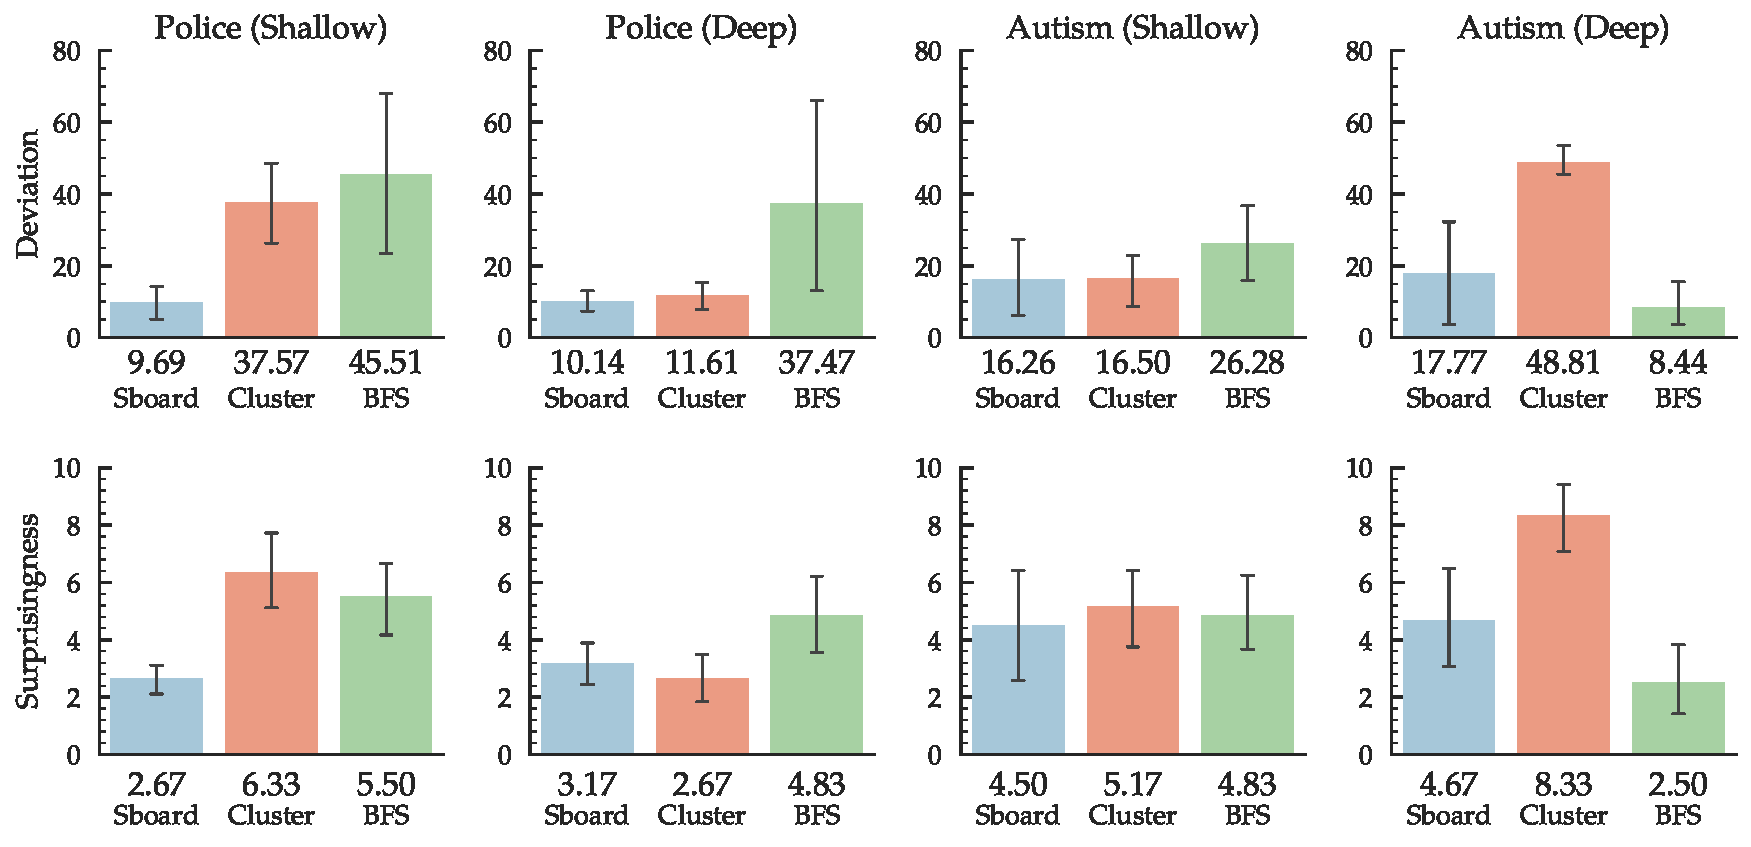
\includegraphics[width=\linewidth]{figures/Devation_Surprisingness.pdf}
\caption{Top: Euclidean distance between predicted and ground truth. Bottom: Surprisingness rating reported by users after seeing the actual visualizations on a Likert scale of 10.}
\label{fig:distance}
\end{figure*}
\begin{figure*}[bht]
\centering
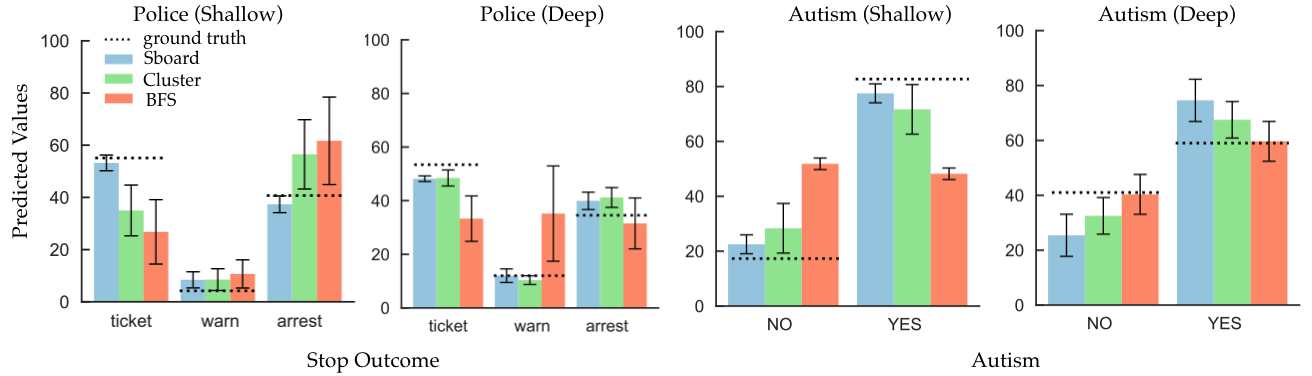
\includegraphics[width=\linewidth]{figures/Prediction_Actual.png}
\caption{Mean and variance of predicted values. Predictions based on \system exhibits lower variance (as indicated by the error bars) and greatly proximity to the actual values (dotted).}
\label{fig:actual_predictions}
\end{figure*}
\subsection{Qualitative results (RQ3)}
We analyzed the transcriptions of the study recordings through an open coding process by two of the authors. For each task performed by the participants, a binary-valued code is assigned to indicate whether or not the participant engaged in the particular event (action or thought process). We will refer to participants engaging in a dashboard created by algorithm=\{1,2,3\}=\{\system, \cluster, \BFS\} on dataset =\{A,B\}=\{Police, Autism\} with the notation [Participant.DatasetAlgorithm].

\stitle{\system promotes distribution-awareness by provoking comparisons against more informative contextual references.}
\par We first examined the thematic codes regarding how participants understood the context of the visualization distribution. In particular, we were interested in the types of visualizations that participants compared against in order to form their expectations regarding how other visualizations should be distributed. We define this property of visualization understanding as \textit{distribution-awareness} and the visualizations that are compared against as the \textit{contextual reference}. Via the thematic coding, we uncovered four main classes of contextual references, described below using the example visualization \texttt{gender=F, race=White, age=21-30} (in order of most to least similar):
\begin{enumerate}
	\item Parent : Comparison against a visualization with one filter criterion removed (e.g. \texttt{gender=F, race=White})
	\item Siblings : Comparison against a visualization that share the same parent. In other words, the filter types are the same, but with one criterion that inherit a different value. (e.g. \texttt{gender=M, race=White, age=21-30})
	\item Relatives : Comparison against a visualization that share some common ancestor (excluding overall), but not necessarily the same parent. In other words, these visualizations share at least one common filter type, but with more than one criterion that inherit a different value. (e.g. \texttt{gender=F, race=White, age=60+, search conducted=T})
	\item Overall : Comparison against the distribution that describes the overall population (no filters applied).
\end{enumerate}
Studying participants' use of contextual reference reveals inherent challenges in dashboard selection through \BFS and \cluster. As shown in Table \ref{table:contextual_reference_count}, participants mainly compared against relatives and the overall. Since \cluster optimizes for diversity of shape distributions amongst the visualization, the selected visualization had up to 4 filters and were disconnected from each other. For this reason, in many cases participants could only rely on relatives and overall as contextual references to gain distribution-awareness. For example, [P4.A2] dislike how ``a lot of [the visualizations] are far too specific. [Pointing at visualization consisting of 4 filters with a 100\% bar for warning] This is not very helpful. You can't really hypothesize that all people are going to be warned, because it is such a specific category, it might just be one person''. %, you need to have a bigger dataset. And that category will not really give you such extremes to make it more credible''.
He further explained how he ``would not want to see the intersections (visualizations with multi-variable filters) at first and would want to see all the bases (visualization with one variable at a time) then dig in from there.'' In addition, the lack of informative contextual reference in the \cluster dashboard is reflected in the high variance and deviation of the predicted visualization results.
%despite our modification to KMeans which picks the visualizations with the least number of filters to show in the dashboard for improving interpretability
%These themes are drawn from user's explanations of how they obtained certain insights or ---- that --different tasks or while interpreting the dashboards. 4 categories :
\begin{table}[h!]\label{table:contextual_reference_count}
\centering
	\begin{tabular}{l|rrrr|r}
	\hline
	 Algorithm   &   Overall &   Parent &   Sibling &   Relative &   Total \\
	\hline
	 \system     &        11 &       12 &         8 &          0 &      31 \\
	 \cluster     &         8 &        4 &         0 &          7 &      19 \\
	 \BFS         &         8 &        0 &         5 &          1 &      14 \\
	\hline
	\end{tabular}
\caption{Number of participants who made use of each contextual parents, summed across the two datasets. Participant behavior shows a similar trend in individual datasets.}
\end{table}
\par For BFS, most comparisons were among overall and siblings. Due to the sequential, level-wise picking approach, in all cases for the \BFS dashboard generated, the overall corresponded to the immediate parent, so they are not explicitly recorded as parent. While the overall and sibling comparisons can be informative, due to the limited budget $k$, not all first-level visualizations were displayed in the dashboard. These incomplete comparisons can result in flawed reasoning, as observed in the Autism shallow prediction task described earlier. In contrast, for \system, users mainly compared against the overall and parents, while some also exploited sibling comparison information to make a less certain guess. We also find that more participants make comparisons in total using \system than compared to \cluster and BFS.

\stitle{Hierarchical layout leads to more natural contextual comparisons compared to table layout.}
\par As described in the previous section, contextual parents are important in establishing distribution-awareness for understanding the dataset. Participants cited hierarchical layout as one of the key reasons why it was easier to follow contextual reference in \system. Based on the hierarchical layout in \system, users were able to easily interpret the meaning of the dashboard, even though they were never explicitly told what the edge connections between the visualizations meant. For example, [P1.A1] stated that ``the hierarchical nature [is] a very natural flow...so when you are comparing, you don't have to be making those comparisons in your head, visually that is very pleasing and easy to follow.'' %Likewise, [P8.A1] also stated that ``I like the different levels, it makes it very visually easy to figure out what you want to look at, if you want to look at the overall data, it's right there at the top for you, if you want to get more specific, you just follow a branch downwards, which I think is very intuitive.''
Likewise, P9 described how the hierarchical layout she saw for the autism dataset was a lot easier to follow than the police dataset shown in the table layout:
\begin{quote}
If I had to look at this dataset in the format of the other one, this would be much more difficult. It was pretty hard for me to tell in the other one how to organize the tree, if there was even a tree to be organized. I like this layout much better, I think this layout allows me to approach it in a more meaningful way. I can decide, what do I think matters more: the overall trend? or the super detailed trends? and I know where to look to start, in the other one, every time I go back to it, I would say, where's the top level, where's the second level? I mentally did this. Like when you asked me that first question, it took much longer to find it, because I literally have to put every chart in a space in my head and that took a lot longer than knowing how to look at it.
\end{quote}
At the end of the study, some participants for \BFS and \cluster sketched and explained how they would like the layout of the visualizations to be done. Participants expressed that they wanted ``groupings'' or layouts that arranged visualizations with the same attribute together. Other participants advocate for isolating the overall visualization outside of the dashboard table for facilitating easier comparisons. Both of these provides further motivation for our hierarchical layout and the idea of the collapsed visualizations as described in Section \ref{sec:interaction}.
\par Since we did not inform participants how the dashboards were generated, it was also interesting to note that some participants thought that the dashboards were hand-picked by a human analyst and described what this person's intentions were (e.g. ``It seems like the researcher who created this dashboard was specifically looking at people of Asian descent and people who are 60 or older.'' [P7.A1]). We encoded this phenomenon by looking at instances where a participant either explicitly referring to a person who picked out the dashboard or implicitly described their intentions through personal pronouns. A total of 5 different participants referred to the dashboard generated by \system as generated by a human, whereas there was only 1 participant for \cluster and none for \BFS made such remarks. At the end of the study, many were surprised to learn that the \system dashboard was actually picked out by an algorithm, indicating that \system could automatically generate convincing dashboard stories that were similar to a dashboard that was authored with intention.

\stitle{Improper contextual reference can lead to misleading insights.}
\par While comparisons are essential for data understanding, choosing the wrong contextual reference for comparison could lead to misleading insights. In particular, when a visualization that is composed of multiple filter conditions is shown in a dashboard created using \cluster, 5 out of 12 participants for both datasets had a hard time interpreting the meaning of the filter, whereas there was only 1 for \system and BFS. This is due to the fact that \cluster dashboards are seemingly random to the users, whereas \BFS and \system both have some natural ordering. In addition, when examining visualization with many filters and contain bars that exhibit extreme values (bars with 100\% or 0\% in one or more categories), 4 \cluster participants did not realize that charts with multiple filters may have a smaller subpopulation size. This issue stems from the fact that the contextual reference used for comparison was the overall population, however the unseen parent subpopulation may have behaved very differently. The fallacy was observed to be more severe for the Autism dataset, where participants had less intuition on the expected attribute behavior. In contrast, 6 of the participants using \system recognized that while these extreme-valued visualizations may be interesting, they were less certain due to the unknown subpopulation size and should be investigated further. For example, [P1.A1] noted that a visualization with warning=100\% caught her eye, ``but I don't know what the N is, maybe it's one person, this makes me a little skeptical, that makes me want to go back to the raw data and look at what is the N and what drives something so drastic?''. Since \BFS dashboards only displayed first-level visualizations, participants for \BFS did not see such visualizations during the study session, so we did not see signs of this fallacy for \BFS participants.

\stitle{Limitations of \system}
\par As described earlier, since the details of how the dashboard was obtained was not explained to the users during the study, some users expressed that they were initially confused by \system since not all variables were present in the dashboard and others found it confusing that the addition of filters did not always correspond to the same variables. For example, [P2.A1] criticized how the dashboard was intentionally selected to be biased:
\begin{quote}
I feel like this one, not all the data is here, so we are already telling a story, you are trying to steer the viewer to look at certain things. And the focus seems to be on where the arrest rate is high. You probably could have found other things that led to ticket being high, but you didn't pull those out. You are trying to see if there are other factors that leads to more arrests.
\end{quote}
\npar This sentiment is related to participants' desire to perform their own ad-hoc querying alongside the dashboard to inspect other related visualizations for verifying their hypothesis. For example, [P7.A1] wanted to inspect all other first-level visualizations for driver's race to assess its influence. [P7.A1] expressed that while he had learned many insights from the dashboard, ``the only thing I don't like is I can not control the types of filter, which is fixed.'' Outside the context of the user study, it is essential to explain how \system are picking the visualizations in a easy and interpretable manner to establish a sense of summarization guarantee for the users and help them make better inferences with the dashboard.
\par As discussed earlier, subpopulation size is important in establishing the `credibility' of a visualization. While subpopulation size is taken into account implicitly in our objective (as described in Section~\ref{sec:utility}), we should design interfaces that can convey the notion of subpopulation size in our dashboard, either explicitly displayed as text when hovering over the visualization or changing the size or background color of the visualizations to encode subpopulation size.
%“I actually found it really confused at first because such a low arrest rate at the top, and then at the bottom the arrest rate was much higher, so I was like is this data wrong. Then I realized we’re not looking at all the data here, you’ve pulled out some of it. It took me a minute to realize that. And once I read the title of the charts I realized that makes sense.” [P2.A1]
% - Reference of Comparison
% - Layout naturally lends itself for comparison:
% 	- describe ordering layout, how participants naturally follow the flow
% 	- emph that we did not tell them what the edge connections mean and how they were computed but the users naturally figured it out, that it means adding an additional filter.
% 	- hierarchical interpretable nature (quotes)
% 	- compared to other baselines
% 	- describe dashboard by human (count)
% - Misleading insights v.s. True insight discovery rates
% 	- Interpretability:
% 	- misled understanding subpopulation size
% 		- for autism, it is important to see if they compare to overall because if not they would think high skew to NO is important whereas its actually pretty close to overall.
% 	- trouble interpreting filter combination
